\chapter{Wymagania i narzędzia}
\label{ch:wymagania-i-narzedzia}
%\begin{itemize}
%	\item wymagania funkcjonalne i niefunkcjonalne
%	\item przypadki użycia (diagramy UML) -- dla prac, w których mają zastosowanie
%	\item opis narzędzi, metod eksperymentalnych, metod modelowania itp.
%	\item metodyka pracy nad projektowaniem i implementacją -- dla prac, w których ma to zastosowanie
%\end{itemize}
Rozdział omawia kluczowe aspekty dotyczące aplikacji do symulowania rozprzestrzeniania się zarażeń o nazwie \textit{InfektoSym}. Rozpocznie się analizy i przedstawienia wymagań funkcjonalnych oraz niefunkcjonalnych. Następnie przybliży technologie wykorzystane w aplikacji. Dodatkowo, dokładnie wyjaśni działanie zaimplementowanego modelu symulacji rozprzestrzeniania się choroby, a także w jaki sposób aplikacja oddziałuje z użytkownikiem i jakie rezultaty może dostarczyć. Ten rozdział stanowi istotne wprowadzenie do zrozumienia zarówno technicznego, jak i funkcjonalnego aspektu projektu.

\section{\textbf{Wymagania funkcjonalne i niefunkcjonalne}}
\subsection{\textbf{Wymagania funkcjonalne}}
\begin{itemize}
	\item \textbf{ Symulacja Ruchu i Interakcji:}
	
	Aplikacja pozwala na śledzenie trajektorii ruchu każdej postaci w biurze w czasie rzeczywistym.
	Interakcje pomiędzy postaciami są symulowane z uwzględnieniem różnych scenariuszy, takich jak rozmowy, wspólna praca, czy przerwy.
	W momencie, gdy jedna postać zostaje zarażona, aplikacja monitoruje, czy i jak szybko choroba rozprzestrzenia się na inne postacie poprzez ich bezpośrednie kontakty.
	\item \textbf{Wizualizacja Stanów Zdrowia:}
	
	Na ekranie widoczne są dynamiczne wskaźniki zdrowia każdej postaci, pozwalające użytkownikowi śledzić ich aktualny stan (zdrowy, narażony, zarażony).
	Symulacja obejmuje także wizualizację okresów inkubacji oraz wyzdrowienia, umożliwiając obserwację zmian stanów zdrowia w czasie rzeczywistym.
	\item \textbf{Monitorowanie Kontaktów i Narażenia:}
	
	Aplikacja zbiera dane dotyczące kontaktów pomiędzy postaciami, identyfikując te, które mogą prowadzić do potencjalnego zarażenia.
	Wizualizacja narażeń obejmuje różne aspekty, takie jak dystans, czas trwania kontaktu oraz ewentualne zastosowane środki ochrony osobistej.
	\item \textbf{Wariacje Scenariuszy:}
	
	Aplikacja umożliwia eksperymentowanie z różnymi scenariuszami zarażenia poprzez dostosowanie parametrów symulacji. Użytkownik może modyfikować takie czynniki jak dystans zarażenia, czas do zarażenia, czy skuteczność maseczek, co pozwala na badanie wpływu tych parametrów na proces rozprzestrzeniania się infekcji w przestrzeni biurowej.

	\item \textbf{Wysoce Parametryzowalna Symulacja:}
	\begin{enumerate}
		\item \textbf{Dystans Zarażenia:}
		
		Użytkownik ma możliwość określenia maksymalnego dystansu, na jakim wirus może się przenosić między agentami.
		\item \textbf{Czas do Zarażenia:}
		
		Określenie czasu, jaki musi upłynąć w bliskim kontakcie z zarażoną postacią, aby doszło do zarażenia.
		\item \textbf{Zaraźliwość Patogenu:}
		
		Parametr definiujący zdolność wirusa do zarażania innych postaci w danym środowisku symulacyjnym.
		\item \textbf{Średni Okres Inkubacji:}
		
		Ustalenie czasu, jaki upływa od momentu zarażenia do pojawienia się objawów u zarażonej postaci.
		\item \textbf{Procent Populacji Noszący Maseczki:}
		
		Możliwość określenia odsetka populacji, który stosuje ochronę w postaci noszenia maseczek.
		\item \textbf{Skuteczność Maseczek:}
		
		Parametr określający, o ile procent zmniejsza się dystans zarażenia dla osób noszących maseczki.
		\item \textbf{Liczebność Populacji:}
		
		Określenie ogólnej liczby postaci uczestniczących w symulacji.
		
		\item \textbf{Początkowy Procent Zarażonych:}
		
		Określenie procentowej liczby zarażonych w początkowej populacji.
		\item \textbf{Odporność Populacji:}
		
		Ustalenie procenta populacji posiadającego naturalną odporność na wirusa.
		\item \textbf{Długość Symulacji:}
		
		Określenie czasu trwania symulacji w jednostkach czasu.
		\item \textbf{Prędkość Symulacji:}
		
		Umożliwienie regulacji prędkości symulacji, włączając przyspieszenie do 100-krotności normalnej prędkości.
		
		\item \textbf{Średni czas wykrycia:}
		
		Ustalenie czasu, jaki upływa od momentu pojawienia się objawów, do ich wykrycia i zlecenia kwarantanny.
		\item \textbf{Pauzowanie Symulacji:}
		
		Dodatkowa funkcjonalność, która pozwala na zatrzymywanie symulacji w dowolnym momencie i jej późniejsze wznowienie.
	\end{enumerate}
\end{itemize}
\subsection{\textbf{Wymagania niefunkcjonalne}}
\begin{itemize}
	\item\textbf{  Intuicyjny Interfejs:}
	
	Interfejs użytkownika powinien być zaprojektowany w sposób intuicyjny, umożliwiając łatwe poruszanie się po aplikacji i korzystanie z jej funkcji. Elementy graficzne, przyciski i opcje powinny być jasne i zrozumiałe dla użytkownika końcowego.
	\item\textbf{ Stabilność:}
	
	Aplikacja powinna charakteryzować się stabilnością działania, eliminując nieoczekiwane błędy, które mogą prowadzić do awarii. Wszystkie funkcje aplikacji powinny działać zgodnie z oczekiwaniami, zapewniając płynne doświadczenie użytkownika.
	\item\textbf{ Odporność na Awarie:}
	
	Aplikacja powinna być odporne na awarie poprzez implementację mechanizmów zabezpieczających, takich jak obsługa błędów, przywracanie stanu aplikacji po awarii, oraz minimalizacja wpływu awarii na całość systemu.
	
	\item \textbf{Płynność Symulacji:}
	
	Aplikacja powinna zapewniać płynną symulację nawet przy dużej ilości agentów uczestniczących w scenariuszu. Optymalizacje i zoptymalizowany kod powinny umożliwiać utrzymanie odpowiedniej prędkości symulacji, niezależnie od skomplikowania scenariusza.
	
	\item\textbf{ Responsywność Interfejsu:}
	
	Interfejs użytkownika powinien reagować szybko na akcje użytkownika, zapewniając natychmiastowe odpowiedzi na interakcje, co przyczyni się do lepszego doświadczenia użytkownika.
\end{itemize}
\section{\textbf{Wybrana technologia}}

Rozważając wybór technologii do stworzenia aplikacji \textit{InfektoSym}, zdecydowano się na silnik gier Unity. Ten wybór był podyktowany kilkoma kluczowymi czynnikami, mającymi istotne znaczenie dla skuteczności i efektywności projektu.

Przede wszystkim, istnienie dużej społeczności użytkowników stanowiło istotny argument. Unity cieszy się uznaniem ze względu na szeroki dostęp do materiałów szkoleniowych wideo, aktywność na forum dyskusyjnych oraz obfite źródła dokumentacji online. Ta społeczność stanowi nie tylko źródło wsparcia, lecz także umożliwia szybsze rozwiązywanie potencjalnych problemów napotkanych podczas procesu tworzenia aplikacji.

Duże możliwości rozwoju były kolejnym czynnikiem decydującym o wyborze Unity. Silnik ten oferuje elastyczność i skalowalność, co pozwala na rozbudowę aplikacji w miarę ewentualnych zmian w wymaganiach projektu.

Aspekt wydajności miał kluczowe znaczenie dla płynności symulacji. Unity, dzięki zoptymalizowanym mechanizmom renderowania i obsługi fizyki, pierwotnie zaprojektowanych do tworzenia gier komputerowych, świetnie odnajduje się w przeprowadzaniu wszelkiego rodzaju symulacji gdzie ważna jest reprezentacja graficzna.

Gotowe narzędzia dostarczane przez Unity, takie jak edytory interfejsu użytkownika czy wbudowany system nawigacji dla poruszających się obiektów, znacząco skracają czas potrzebny na rozwój aplikacji. To ułatwienie pozwala skupić się na kluczowych aspektach projektu.

Podsumowując, wybór Unity jako platformy do tworzenia \textit{InfektoSym} wynikał z korzyści płynących z bogatego ekosystemu, wydajności silnika oraz dostępności narzędzi ułatwiających pracę, co zapewniło efektywny i skuteczny proces realizacji projektu.
\section{\textbf{Model symulacji rozprzestrzeniania się zarażeń zastosowany w InfektoSym}}

Model symulacji zaimplementowany w \textit{InfektoSym} stanowi połączenie modelu SEIR z podejściem opartym na agentach, mając na celu dokładne odwzorowanie rozprzestrzeniania się zarażeń. Struktura modelu zakłada podział populacji na cztery główne grupy, analogiczne do SEIR:
\begin{itemize}
	\item \textbf{Zdrowi (Susceptible)}  - grupa osób zdrowych.
	\item \textbf{Narażeni (Exposed)} - grupa osób, które miały kontakt z zarażonym i są potencjalnie podatne na zakażenie.
	\item \textbf{Zarażeni (Infected)} - grupa osób, u których choroba jest aktywna, co stanowi źródło dalszego zarażania.
	\item \textbf{Usunięci (Removed)} - osoby, które zostały zidentyfikowane jako chore i zostały odizolowane.
\end{itemize}
Symulacja opiera się na podejściu agentowym, skupiając uwagę na indywidualnych decyzjach każdego z osobników. Ten szczególny nacisk na indywidualność umożliwia uchwycenie subtelności wprowadzanych przez decyzje jednostki, co jest istotne dla precyzyjnego modelowania dynamiki rozprzestrzeniania się zarażeń.

\subsection{\textbf{Równania opisujące model symulacji}}
Założenia modelu oraz parametry symulacji pozwalają wyizolować równania opisujące prawdopodobieństwo zarażenia w określonych warunkach.

Przejście agenta ze stanu zdrowego do narażonego obliczane jest według następujących parametrów i równań:

Jeżeli zdrowa osoba przebywa w odległości $x < d_{maks}$, gdzie $x$ to odległość od zarażonego, a $d$ to maksymalny dystans, na jaki patogen może się przenosić w czasie $t_k > t_z$, gdzie $t_k$ to czas kontaktu, a $t_z$ to minimalny czas potrzebny do zakażenia. Szansa na przeniesienie do grupy narażonych (exposed) określana jest przez parametr zdolności zarażania patogenu $R_0$ (jeżeli $R_0 = 50$, przy każdym kontakcie szansa na narażenie wynosi 50\%).
Dodatkowymi parametrami grającymi tu rolę jest posiadanie maseczki i jej skuteczność. Dystans przenoszenia się patogenu jest procentowo zmniejszany w zależności od ustawionej skuteczności maseczek.\\

Kiedy agent zostanie uznany za narażonego, program wylicza procentowe szanse na rozwój choroby. Na podstawie wzoru:

\begin{center}
	$P_z = R_0 \cdot (1 - I)$
\end{center}

gdzie:\\
$P_z \in <0,100> $ - szansa na zostanie zarażonym, wyrażona w \% \\
$R_0 \in <0,100>$ - współczynnik zakażalności patogenu \\
$I \in <0,1>$ - odporność jednostki.\\

Wykonywane jest losowanie; jeżeli tak, osobnik zostanie przeniesiony do grupy zarażonych (Infected), jeżeli nie, wróci do puli zdrowych (Susceptible). W obu przypadkach stanie się to po czasie $T_{inkubacji} \pm 24$ godziny (czasu symulacji).

Osoba zakażona jest usuwana z symulacji po czasie $T_{wykrycia} \pm 24$ godziny (czasu symulacji).

\begin{figure}[h!]
	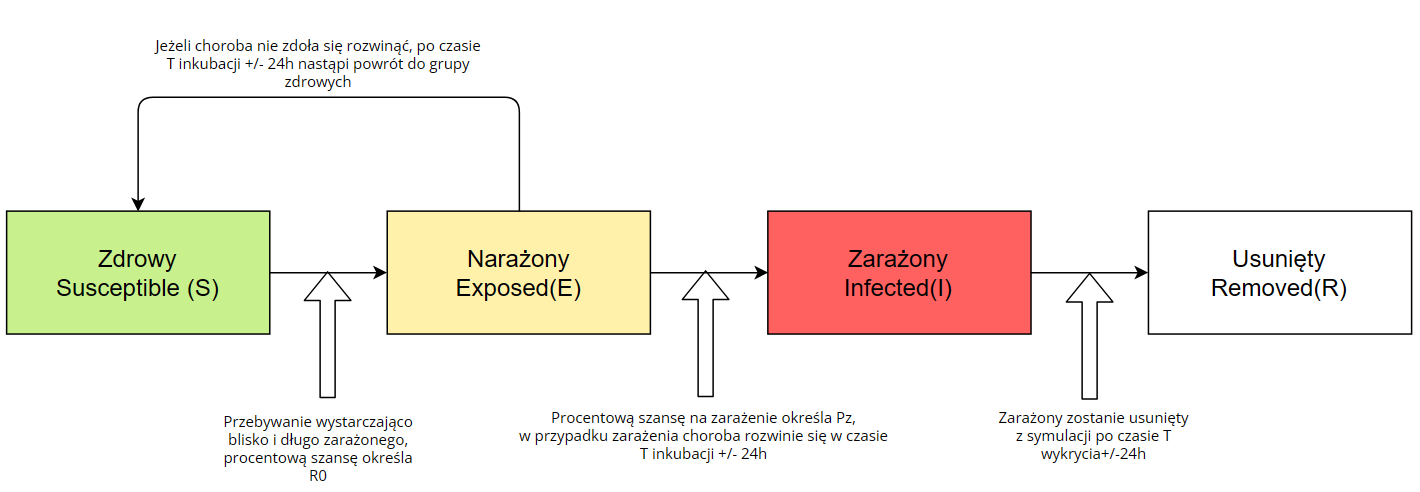
\includegraphics[width=\linewidth]{diagramModelu.png}
	\caption{Schemat działania modelu użytego w \textit{InfektoSym}}
\end{figure}

\subsection{\textbf{Symulacja zachowań ludzkich}}
W ramach symulacji zachowań ludzkich w aplikacji, agenci mają zdefiniowane konkretne czynności, które mogą wykonywać. Poniżej przedstawiono proces realizacji tych aktywności (poniższe wartości czasowe odnoszą się do czasu symulacji):

\begin{itemize}
	\item \textbf{Początkowe Losowanie:}
	\begin{itemize}
		\item Kiedy agent pojawiając się w symulacji, losuje jedną z czterech podstawowych akcji: losowe spacerowanie, praca, przerwa lub lunch.
		\item Każda akcja(oprócz losowego spacerowania) trwa od 1 do 4 godzin.
	\end{itemize}
	
	\item \textbf{Zmiana Akcji:}
	\begin{itemize}
		\item Po zakończeniu aktualnej akcji, agent wybiera nową spośród losowego spacerowania, pracy, przerwy lub lunchu.
		\item Ten proces powtarza się, co pozwala agentowi na cykliczne zmiany działań.
	\end{itemize}
	
	\item \textbf{Rozmowy:}
	\begin{itemize}
		\item Kiedy agenci się mijają, mają 4\% szansę na rozpoczęcie rozmowy.
		\item Rozmowa trwa od 10 minut do 1 godziny, a po jej zakończeniu agent wybiera nową akcję.
	\end{itemize}
	
	\item \textbf{Praca, Odpoczynek i Lunch:}
	\begin{itemize}
		\item Jeśli agent zdecyduje się pracować, odpoczywać lub coś zjeść sprawdza dostępność odpowiednio biurek, miejsc na kanapie, stolików w kuchni.
		\item Siada przy pierwszym wolnym miejscu i wykonuje czynność od 1 do 4 godzin, po czym wybiera nową akcję.
		\item W przypadku braku wolnych miejsc agent rozpoczyna losowe spacerowanie.
	\end{itemize}
\end{itemize}

Ten proces symulacyjny pozwala na odwzorowanie różnorodnych działań agentów, obejmujących pracę, odpoczynek, jedzenie i społeczne interakcje. Losowanie czasu trwania i zmiana akcji wprowadza naturalność w zachowaniach agentów.



